\chapter{Softwarewijzigingsproces}
Van software in 2018 wordt verwacht dat deze constant geupdate blijft met onder andere nieuwe features en security patches.
Om te zorgen dat dit proces goed verloopt geeft dit hoofdstuk weer hoe een verandering aan de software gemaakt kan worden.
Er wordt uitgegaan van enige ontwikkelaarskennis aangezien iemand die een verandering maakt bekend moet zijn met software ontwikkeling.

\section{Wijzigingsverzoeken van een externe partij}
\begin{figure}[H]
	\centering
	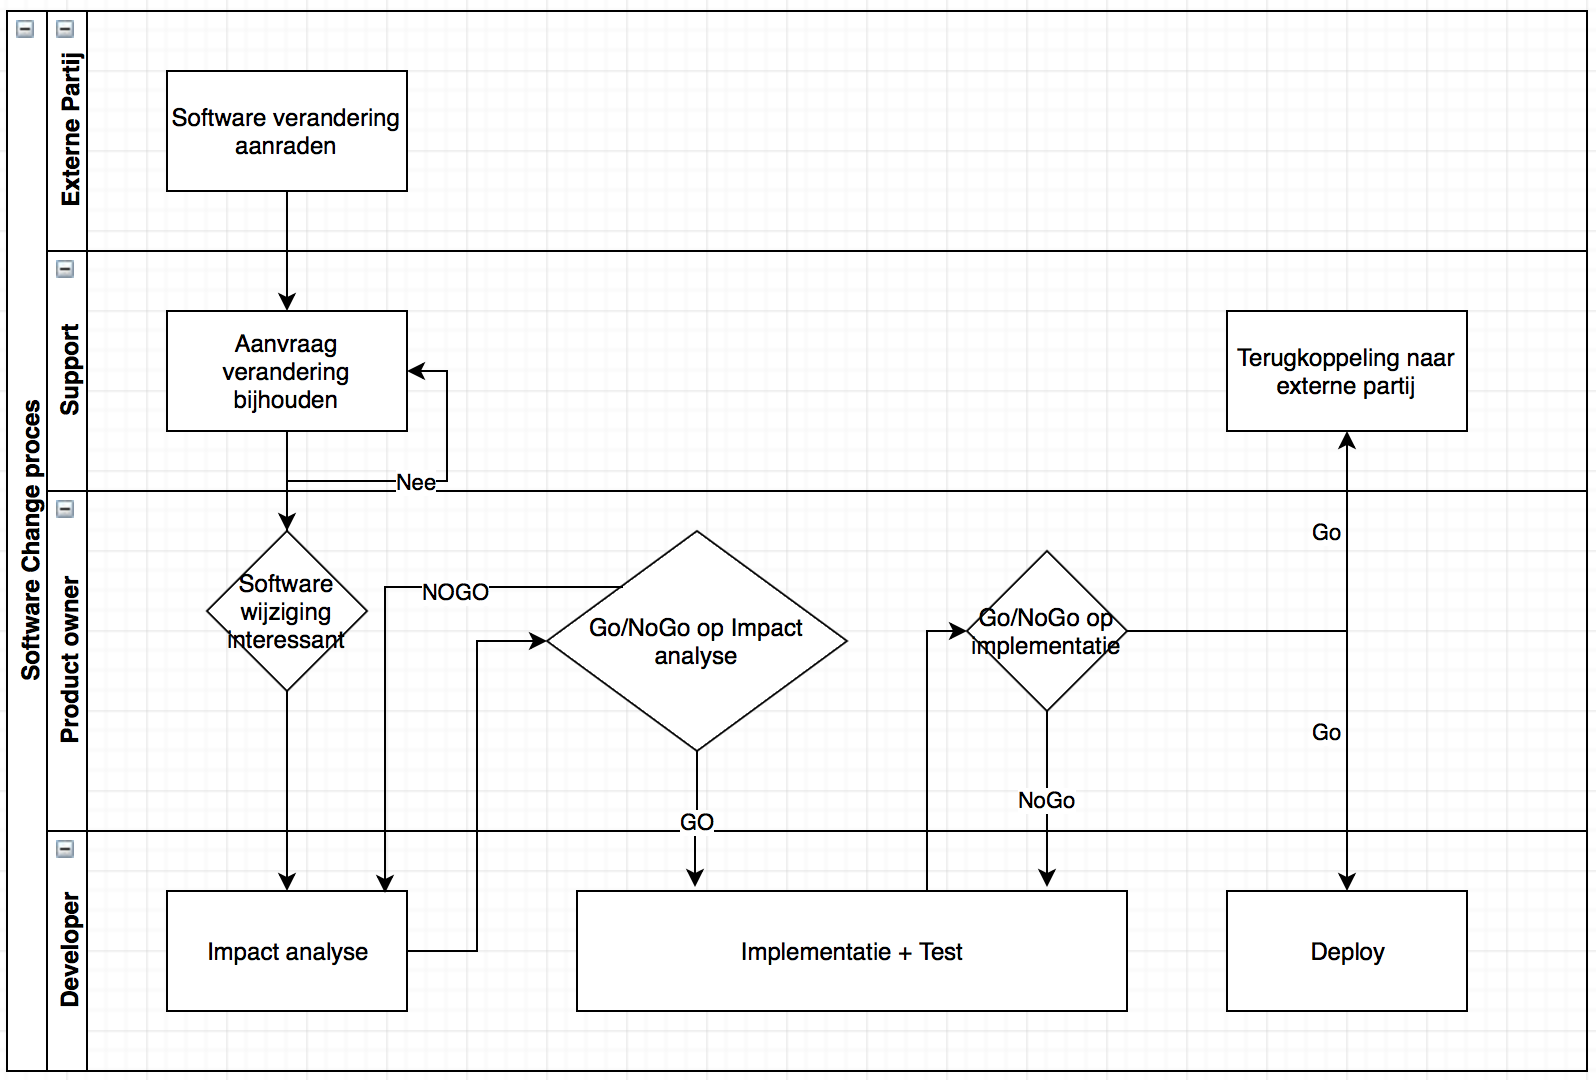
\includegraphics[width=0.95\textwidth]{images/ChangeRequest.png}
	\caption{Flowchart voor het afhandelen van een change request}
	\label{fig:ChangeRequest}
\end{figure}

\subsection{Rol van de externe partij}
De externe partij is een breedt begrip. Dit kunnen zowel gebruikers van de applicatie zijn, maar ook evenetuele ontwikkelaars van frameworks die gebruikt worden binnen een applicatie.

De externe partij zorgt ervoor dat er nieuwe aanvragen worden gedaan voor wijzigingen in de software. Dit kunnen aanvragen zijn voor nieuwe functionaliteiten, maar ook aanvragen om eventuele bugs op te lossen. Denk hierbij bv. aan foute berekeningen, of worden die niet correct vertaald zijn.

\subsection{Rol van de Support}
De support rol zorgt ervoor dat de verschillende aanvragen juist worden bijgehouden, en dat er meer informatie bij komt om de aanvraag zo duidelijk mogelijk te hebben. Elke nieuwe aanvraag wordt voorgesteld aan de Product owner, deze kan er dan voor zorgen dat de nieuwe functionaliteit wordt geïmplementeerd.

\subsection{Rol van de Product Owner}
Wanneer de product owner vanuit de support rol een nieuwe verandering krijgt aangeboden, wilt hij deze laten analyseren door een software ontwikkelaar. Door de verandering te laten analyseren, is het voor de product owner duidelijk wat de verwachte impact zal zijn van de wijziging in de software. Door middel van verschillende Go/NoGo momenten kan de product owner duidelijkheid krijgen over de voortgang van het veranderingsverzoek.
Mocht een verandering geaccepteerd zijn, dan kan de product owner dit terug koppelen naar de support rol. Op deze manier zou de support rol dit terug kunnen koppelen naar de aanvrager van de wijziging.

\subsection{Rol van de ontwikkelaar}
De ontwikkelaar heeft de taak om de wijziging door te voeren in de software. Voordat hij/zij hiermee begint, zal er eerst een impact analyse uitgevoerd worden. Aan de hand van deze analyse kan geschat worden wat de impact van de wijziging zal hebben op de software.
Wanneer deze analyse is voltooid en terug gekoppeld is aan de product owner volgt hier een Go of NoGo uit. Wanneer de analysy geaccepteerd wordt, kan de ontwikkelaar beginnen aan de implementatie van de wijziging.
Hoe deze implementatie afgehandled wordt staat beschreven in hoofdstuk \ref{hfd:wd}. Wanneer de implementatie voltooid, getest en geaccepteerd door de product owner is, kan de nieuwe wijziging beschikbaar worden gestelt voor de gebruikers. Op dit punt kant tevens de product owner terugkoppeling geven naar de support rol.
\newpage
\section{Wijzigingen verwerken door een ontwikkelaar} \label{hfd:wd}
Onderstaande hoofdstukken geven een beeld hoe een ontwikkelaar een nieuw wijzigings verzoek kan uitvoeren.
Veel van onderstaande informatie wordt doorheen dit document in meer detail uitgelegd. 
\subsection{Een eigen branch in Git}
De applicatie staat in het versiebeheer systeem Git, met Git is er de mogelijkheid om geisoleerd van andere veranderingen een wijziging te maken, dit heet dan een branch. 
Zoals uitgelegd in \cref{hfd:vcs} komt elke nieuwe wijziging normaal gesproken in een nieuwe branch (tenzij dit een hotfix is).
Je kan naar een nieuwe branch wisselen met het commando \textit{git checkout -b DEV-(naam)}.
Op deze manier komt de structuur eruit te zien zoals in \cref{fig:BranchScheme}.
In deze branch kun je vervolgens ongestoord je verandering maken.

\subsection{Mergen via een pullrequest}
Nadat je klaar bent met ontwikkelen van je feature kun je de unittests uitvoeren en eventueel aanpassen of maken als dit nodig is.
Als deze slagen kan je een pull request maken, met een pull request kunnen anderen jouw verandering bekijken voordat zij deze daadwerkelijk toevoegen aan de codebase.
Een pull request geeft ook de mogelijkheid te discussieren over de nieuwe code.
Een pull request moet eerst goedkeuring krijgen van een ander lid binnen het ontwikkelteam om deze toe te voegen aan de development branch.
\begin{figure}[h]
	\centering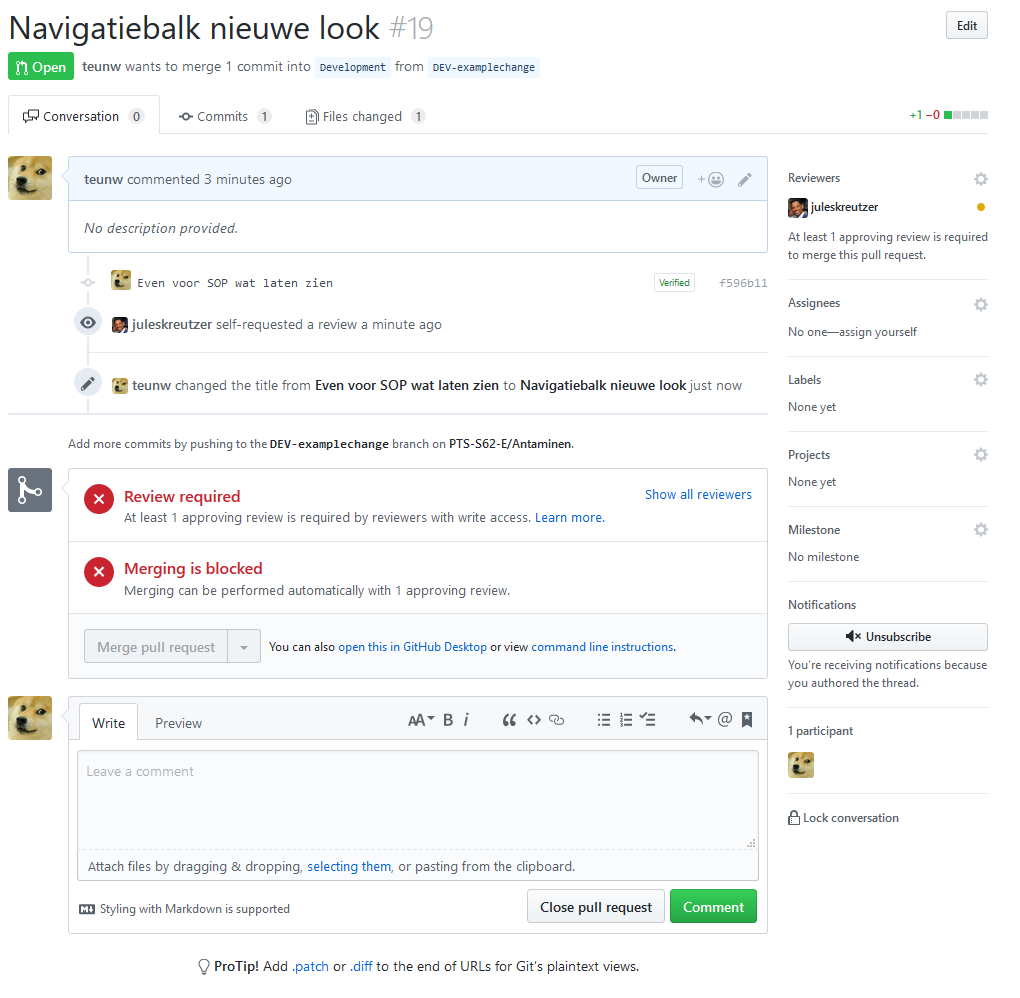
\includegraphics[width=0.6\textwidth]{images/PullRequestExample.png}
	\caption{Een voorbeeld pull request}
\end{figure}

\subsubsection{Tests}
Binnen Jenkins is het mogelijk om te kijken of tests voor jouw pull request slagen.
Dit is belangrijk, omdat falende tests een fout in de tests of codebase betekenen.
Op Github is geen mogelijkheid om een request tegen te houden als tests niet slagen, het is dan ook de verantwoordelijkheid van ontwikkelaar en reviewer(s) om te kijken of tests geslaagd zijn.
Als een test niet slaagt, is het de verantwoordelijkheid van de ontwikkelaar van de code om dit te repareren.

\subsection{Acceptatietesting via staging branch}
Nadat de veranderingen uit de development branch zijn ge-unittest en afgerond zijn (bijv. aan het einde van een sprint) kan de development branch gebouwd worden, deze wordt dan neergezet in de staging omgeving. De code wordt binnen de development branch ook naar de staging branch gezet.
Binnen de staging omgeving wordt er gekeken of:
\begin{itemize}
	\item Er voldaan is aan de user stories, volgens de definition of done (zie \cref{sec:dod}).
	\item De stakeholders tevreden is met het resultaat.
	\item Of de veranderingen kunnen worden gedeployed op de productieomgeving.
\end{itemize}

\subsection{In productie}
Zodra aan de bovenstaande voorwaarden is voldaan kan de staging branch naar productie gepushed worden.
\par
Bij het pushen naar productie wordt niet meer de code uit Git gebruikt, in plaats hiervan wordt de build van de applicatie in de staging omgeving gebruikt.
Dit zorgt ervoor dat de applicatie precies hetzelfde blijft en er dus minder kans is dat een stuk geteste code een fout vertoont.
\par
Binnen de productie branch kan niet direct gepushed worden, maar merge requests kunnen er wel naartoe gemaakt worden, eventueel als hotfixes. Hotfixes worden toegepast wanneer er een kritieke fout in de applicatie is ontdekt, zodat deze fout zo snel mogelijk gerepareert is.
Een hotfix gaat vaak ook niet door het normale proces heen, maar wordt direct naar productie gepushed zodat gebruikers zo snel mogelijk verder kunnen.

\clearpage
\subsection{Overzicht}
Om het stappenplan wat duidelijker uit te beelden is het onderstaande diagram getekend. Dit diagram geeft samenvatting in het ontwikkelen van een nieuwe feature vanaf het begin tot aan het mergen in de productie omgeving.
\begin{figure}[h]
	\centering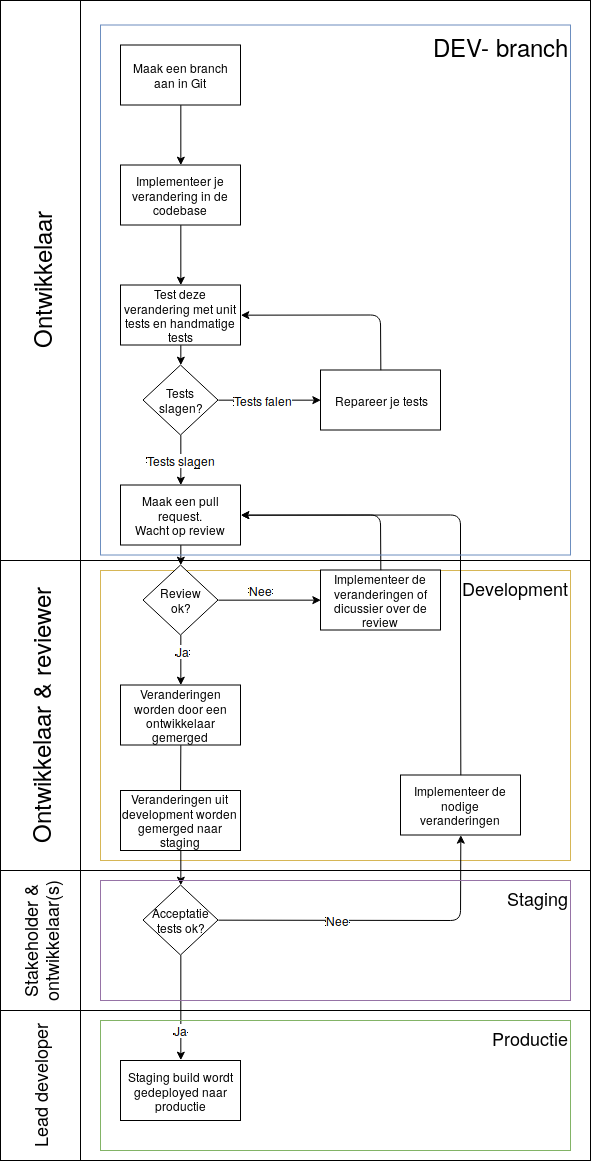
\includegraphics[width=0.56\textwidth]{images/UMLSoftwareChange.png}
	\caption{Het softwarewijzigingsproces als UML diagram}
\end{figure}